paragraph{More Examples : }

Finally with regard to data dependencies alone, we consider
the following code excerpt.

\begin{verbatim}

00	r2 <- r0 op r1
10	r3 <- r2 op r0
20	r2 <- r0 op r4
30	r5 <- r2 op r4

\end{verbatim}

In this example we will put together some of the
code execution and data dependency rules already illustrated
separately.
We assume that after all of the above instructions are loaded
that instruction 10 gets to execute first.
Next, instructions 00 and 30 get to execute together in a single
clock.  Instruction 00 then broadcasts an update for register
{\tt r2}.
This enables or re-enables instructions 10 and 30 to execute again.
They do so in the next clock cycle.  Next, instruction 20 finally
gets a chance to execute.  Again an update for register
{\tt r2}
is broadcast forward.  This enables instruction 30 to execute again
but not instruction 10.
Finally, instruction 00 executes again for some reason.
Again, an update for register
{\tt r2}
is broadcast forward.  However, this update does not enable
instruction 30 to execute again since it had previously used
a value from instruction 20.  At the same time, this broadcast does
enable instruction 10 to execute again and it does so in the following
clock cycle.

The time order of these executions is shown in
Figure~\ref{ex4}.

\begin{figure}
\centering
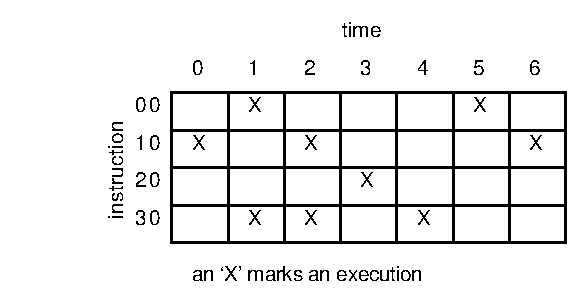
\epsfig{file=e4.eps,width=2.50in}
\caption{{\em Timing of the code example, scenario 4.}
In this example an output data broadcast from instruction 00
in time cycle 4 enables one later instruction to
execute but not one later still in the program order.
Execution of an instruction at a given time is
again indicated by an `X'.}
\label{ex4}
\end{figure}



